% Introduction

% Main chapter title
\chapter{ Hardware Implementation of the algorithms }

% Change X to a consecutive number; for referencing this chapter elsewhere, use \ref{ChapterX}
\label{Chapter8} 

% This is for the header on each page
\lhead{Chapter 7. \emph{Hardware Implementation of the algorithms \& Results}}

The algorithms are written in Aa language. The Aa description is then converted into vhdl using AHIR-tool-chain.\cite{8}


\section{Results}
The designs are characterised by two parameters. First parameter is number of clock cycles required to complete the decoding process or the time required to complete one iteration of decoding. Second parameter is the hardware required to implement the design. By this way we can compare the designs and opt a better trade off between cost verses performance.


 \begin{figure}[h]
 \begin{center}
    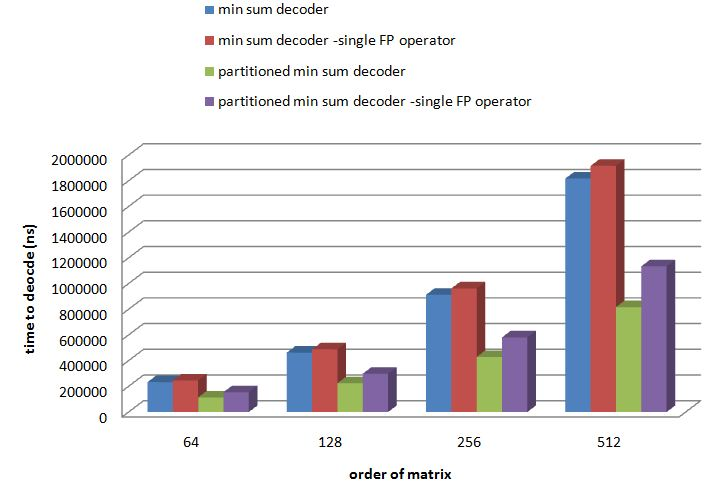
\includegraphics[height=8cm,width=12cm]{result_time.jpg}
    \caption{Comparison of time taken to decode} 
    \label{result_time}
 \end{center}
\end{figure}


Figure \ref{result_time} shows the time taken to decode for all the implemented designs for various order of matrices. The matrices used are randomly generated parity check matrices. The code rate is taken as half. Figure \ref{result_time} concludes that partitioned min sum decoder can decode approximately at half the time as compared to min sum decoder. \\
A floating point operation is very costly. Thus to reduce the cost of hardware we can also use single floating point operator. Its a trade off between cost verses performance. Figure \ref{result_time} shows that, if for both decoders we use shared floating point operator then the time to decode increases.  
 \begin{figure}[h]
 \begin{center}
    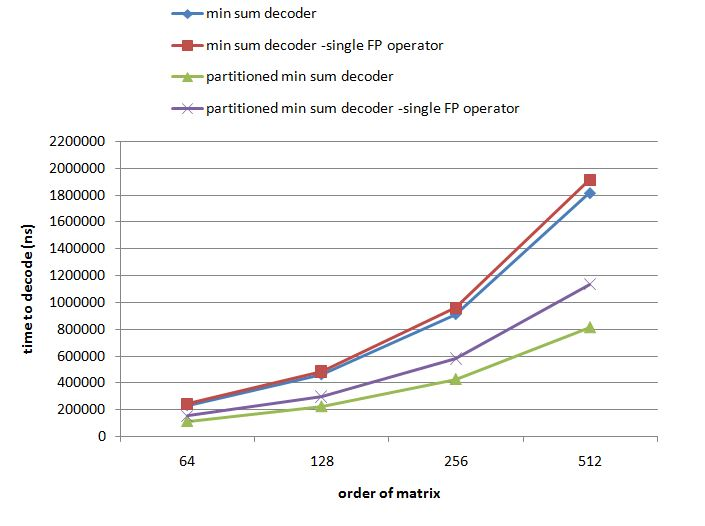
\includegraphics[height=8cm,width=12cm]{result_time1.jpg}
    \caption{Timing trends as the function of order of matrix} 
    \label{result_time1}
 \end{center}
\end{figure}

Figure \ref{result_time1} shows the variation of time to decode as the function of order of matrix. This concludes that the time to decode increases linearly with the order of matrix. \\


The hardware to implement the designs can be compared using Table \ref{result_hw}

\begin{table}[H]
\centering
\caption[Comparison of  hardware generated after implementing the designs]{ Comparison of  hardware generated after implementing the designs }
\begin{tabular}{|p{1.3cm}|p{3.5cm}|p{3.5cm}|p{3.5cm}|p{3.5cm}|}
\hline
	& min sum decoder & min sum decoder \newline
	(single FP unit) & partitioned min sum decoder & partitioned min sum decoder(single FP unit) \\ \hline
FF & 18,076		&19,034		&49,854		&55,988 \\ \hline
LUT & 19,502  &20,621 &  51,929 & 60,296 \\ \hline
Memory LUT & 6 & 3 & 23 & 2 \\ \hline 
I/O & 128 & 128 & 128 & 128 \\ \hline
BRAM & 56 & 56 & 80 & 80 \\ \hline
BUFG  & 1 & 1 & 1 & 1 \\ \hline
\end{tabular}
\label{result_hw}
\end{table}

 \begin{figure}[h]
 \begin{center}
    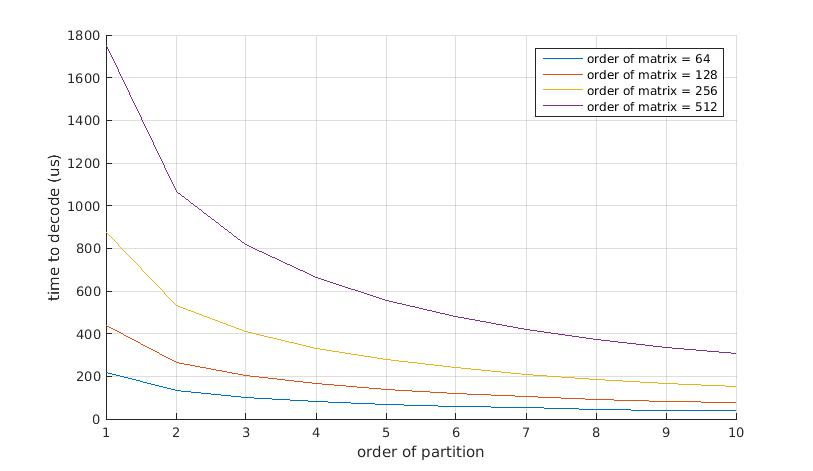
\includegraphics[height=8cm,width=12cm]{untitled.jpg}
    \caption{Timing trends as the function of order of partition} 
    \label{untitled}
 \end{center}
\end{figure}

Figure \ref{untitled} shows the time to decode the code block as a function of order of partitioning. The plot shows that for n-way partitioning of parity check matrix the time to decode reduce by a factor of n. The matrix used are random and have rate of half.


